\documentclass{article}

\usepackage{caption}

\usepackage{multirow}

\usepackage{graphicx}
\setlength{\abovecaptionskip}{10pt plus 3pt minus 2pt}
\setlength{\belowcaptionskip}{10pt plus 3pt minus 2pt}

\usepackage[margin=1in]{geometry}

\usepackage{hyperref}
\hypersetup{
    pdfborderstyle={/S/U/W 1},
    colorlinks=true,
    linkcolor=blue,
    filecolor=magenta,
    urlcolor=cyan,
}

\usepackage{algorithm,algpseudocode}

\usepackage{xcolor}
\usepackage{listings}
\lstdefinestyle{DOS}{
    backgroundcolor=\color{lightgray},
    basicstyle=\scriptsize\color{black}\ttfamily
}

\title{
CSE 5441 (Fall 2019, Dr. Jones)\\
\large POSIX Threads AMR (Lab 2)
}
\author{
Caleb Lehman \\
\href{mailto:lehman.346@osu.edu}{lehman.346@osu.edu}
}

\begin{document}
\maketitle

\section*{Overview}
\label{sec:overview}

For this lab, I modified the previous serial \texttt{C} program to perform
Adapetive Mesh Refinement (AMR)\footnote{See previous lab or project
descriptions for details about AMR computation.} to work in parallel using the
POSIX Threads (\texttt{pthreads}) library. I created two programs,
\texttt{disposable} and \texttt{persistent}, which employ different strategies
for thread creation and destruction (see \textbf{TODO} hyperref [] {}). I
tested these programs on two test files with different numbers of therads to
compare performance against the serial version and against each other.

\subsection*{Results Summary}
\label{subsec:results-summary}

As expected, the \emph{persistent threads} model outperformed the
\emph{disposable threads} model, most likely due to less overhead from not
destroying and recreating threads each iteration. Both parallel programs
outperformed the serial version (at least for optimal choices of number of
threads).

\begin{itemize}

    \item The optimal number of threads for the smaller test case
    (\texttt{testgrid\textunderscore 400\textunderscore 12206}) was 6 for both
    programs.

    \item The optimal number of threads for the larger test case
    (\texttt{testgrid\textunderscore 1000\textunderscore 296793}) was $\sim$20
    for both programs.
    
    \item At the optimal numbers of threads, the \texttt{disposable} program
    was 1.9x faster than the serial program on the small test case and 9.2x
    faster on the large test case.

    \item At the optimal numbers of threads, the \texttt{persistent} program
    was 2.9x faster than the serial program on the small test case and 10.9x
    faster on the large test case.

\end{itemize}

I used all 4 timing methods from lab 1 to collect timing data. All the timing
results I show in this report were collected from \texttt{clock\textunderscore
gettime}. Of particular note is that the \texttt{clock} function from the
\texttt{"time.h"} header is not particulary useful for our purposes, as it
reports CPU time, not wall time. As a result, it consistently returns a
significantly longer time than the actual time the program took to run.

See the \textbf{TODO} section for a more detailed discussion of the results.

\newpage
\section*{Pseudocodes}
\label{sec:pseudocoes}

\subsection*{\emph{Disposable Threads} Model}

Given $\alpha$, $\varepsilon$, a description of grid-aligned boxes, initial
Domain Specific Values (DSV), and a number of threads, the rough pseudocode for
my implementation following the \emph{disposable threads} model is as follows:

\begin{algorithm}
\begin{algorithmic}[1]
\Procedure{Disposable}{$\alpha$, $\varepsilon$, $N$, $Boxes$, $Initial DSV$, $nthreads$}
\State $DSV \gets Initial DSV$, $DSV' \gets Initial DSV$
\While{$(\max{DSV} - \min{DSV})$ / $\max{DSV} > \varepsilon$} \label{alg:amr:convergence}
    \State Create $nthreads$ threads
    \ForAll{$threads$}
        \State \Call{Worker}{$\alpha$, $\varepsilon$, $N$, $Boxes$, $Initial DSV$, $nthreads$}
    \EndFor
    \State Join and destroy all threads
    \State $DSV \gets DSV'$ \label{alg:amr:commit}
\EndWhile
\EndProcedure
\Procedure{Worker}{$\alpha$, $\varepsilon$, $N$, $Boxes$, $Initial DSV$, $nthreads$}
    \State $tid \gets$ current thread number
    \ForAll{$i \in [ tid\cdot \frac{N}{nthreads}, (tid + 1)\cdot \frac{N}{nthreads} ]$}
        \State $DSV'[i] \gets (1 - \alpha)\cdot DSV[i] + \alpha \cdot \sum_{j\in nhbr} DSV[j]\cdot \Call{Overlap}{i, j, Boxes}$
    \EndFor
\EndProcedure
\end{algorithmic}
\end{algorithm}

To summarize, under this model, threads are created at the beginning of each
iteration and execute updates in parallel. Then the threads are joined and
destroyed and the updates are committed.

\subsection*{\emph{Persistent Threads} Model}

Given $\alpha$, $\varepsilon$, a description of grid-aligned boxes, initial
Domain Specific Values (DSV), and a number of threads, the rough pseudocode for
my implementation following the \emph{persistent threads} model is as follows:

\begin{algorithm}
\begin{algorithmic}[1]
\Procedure{Persistent}{$\alpha$, $\varepsilon$, $N$, $Boxes$, $Initial DSV$, $nthreads$}
\State $DSV \gets Initial DSV$, $DSV' \gets Initial DSV$
\State Create $nthreads$ threads to execute \Call{Worker}{$\alpha$, $\varepsilon$, $N$, $Boxes$, $DSV$, $DSV'$, $nthreads$}
\State Join and destroy all threads
\EndProcedure
\Procedure{Worker}{$\alpha$, $\varepsilon$, $N$, $Boxes$, $DSV$, $DSV'$, $nthreads$}
    \State $tid \gets$ current thread number
    \State $range \gets [ tid\cdot \frac{N}{nthreads}, (tid + 1)\cdot \frac{N}{nthreads} ]$
    \While{$(\max{DSV} - \min{DSV})$ / $\max{DSV} > \varepsilon$}
        \ForAll{$i \in range$}
            \State $DSV'[i] \gets (1 - \alpha)\cdot DSV[i] + \alpha \cdot \sum_{j\in nhbr} DSV[j]\cdot \Call{Overlap}{i, j, Boxes}$
        \EndFor
        \State \texttt{BARRIER} to sync all threads
        \State $DSV[range] \gets DSV'[range]$
        \State \texttt{BARRIER} to sync all threads
    \EndWhile
\EndProcedure
\end{algorithmic}
\end{algorithm}

To summarize, under this model, threads are created at the beginning of the
program and destroyed at the end. The threads run in parallel, updating each of
their blocks of DSVs. The threads must be synchronized twice per iterations: 1)
after computing the updates and 2) after commiting updates.

\section*{Tests}
\label{sec:tests}

\subsection*{Environment}
\label{subsec:environment}

The program was developed and tested on a single, 40-core node of the
\href{https://www.osc.edu/resources/technical_support/supercomputers/pitzer}{Pitzer
cluster} at the \href{https://www.osc.edu/}{Ohio Supercomputer Center}.

For development, I loaded the \texttt{intel/18.0.3} module, which allowed the
program to be compiled with version 18.0.3 of the \texttt{icc} C-compiler. I
linked against the \texttt{librt} and \texttt{libpthread} libraries.

For testing, I loaded the \texttt{python/3.6-conda5.2} module, which loads a
python environment with the \texttt{NumPy}, \texttt{SciPy}, and
\texttt{Matplotlib} packages, amoung others.

\subsection*{Timing}
\label{subsec:timing}

I collected timing data using the same 4 methods as the first lab:
\texttt{time}, \texttt{clock}, and \texttt{clock\textunderscore gettime} from
the \texttt{"time.h"} header; and the \texttt{UNIX} utility \texttt{time}.

I didn't use the results from the \texttt{clock} function from the
\texttt{"time.h"} header, since it reports CPU time, not wall time. The other
methods all returned values within 1 second of each other. The \texttt{time}
function declared in \texttt{"time.h"} returns an integer number of seconds,
but the other two methods return with sub-second precision.  \emph{For
consistency, I used the \texttt{clock\textunderscore gettime} function for all
results in this report}.

\subsection*{Test Files}
\label{subsec:test_files}

Dr. Jones provided the \texttt{testgrid\textunderscore 400\textunderscore 12206} test file.
As part of lab 1, I reduced the $\alpha$ (affect rate) and $\epsilon$ parameters until the
serial runtime increased into the 3 to 6 minute range. In particular, I selected $\alpha = 0.01$ and $\epsilon = 0.02$,
for which the serial program completed in 261 seconds.

The above approach of changing the $\alpha$ and $\epsilon$ parameters allows us
to make the programs run longer, but doesn't affect the actual length of each
iteration. With only 12206 boxes, each iteration is fairly short \textbf{TODO},
so it is expected the overhead of synchronizing threads would inhibit
parallelizing beyond a small number of threads. In order to investigate this,
I generated another test file, \texttt{testgrid\textunderscore 1000\textunderscore 12206}, \textbf{TODO}.

\newpage
\section*{Results}
\label{sec:results}

\begin{minipage}{\linewidth}
    \centering
    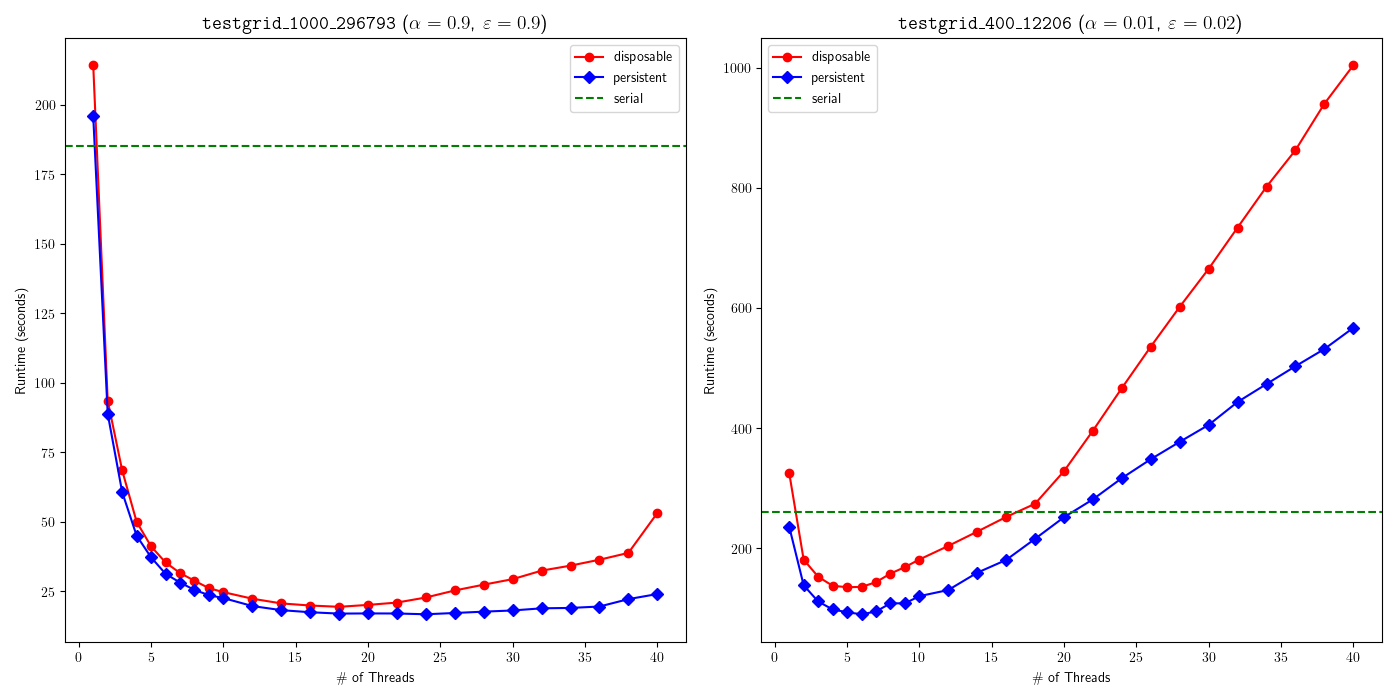
\includegraphics[width=\linewidth]{../results/tests_results.png}
    \captionof{figure}{The runtimes of the parallel versions of the program
    plotted against the number of threads used. Serial runtime is included for
    comparison.}
    \label{fig:runtimes}
\end{minipage}

\section*{Project Usage}
\label{sec:project}

\subsection*{Building}
\label{subsec:building}

To build the \texttt{amr} executable, navigate to the top level of the
submitted directory and build as follows:

\begin{lstlisting}[style=DOS]
# Ensure that you have icc compiler

$ make
...
$ ls
... disposable persistent ...
\end{lstlisting}

\subsection*{Running}
\label{subsec:running}

The syntax to run the program is:

\begin{lstlisting}[style=DOS]
$ ./[program] [affect-rate] [epsilon] [num-threads] <[test-file]
\end{lstlisting}

where \texttt{program} is one of the built programs and \texttt{num-threads} is
an positive integer number of threads.

\end{document}
